%\documentclass[12pt,a4paper]{report}
%\usepackage[utf8]{inputenc}
%\usepackage{amsmath}
%\usepackage{amsfonts}
%\usepackage{amssymb}
%\usepackage[margin=2.5cm]{geometry}
%\usepackage{graphicx}
%\usepackage{caption}
%\usepackage{subcaption}
%\usepackage[nottoc,numbib]{tocbibind}
%\linespread{1.3}
%
%\DeclareMathOperator\arccosh{arccosh}
%\DeclareMathOperator\sgn{sgn}
%
%\begin{document}
\chapter{WKB Potential Barrier}
\label{WKB Potential Barrier}
		In this chapter the derivation of equations used in \cite{b30,b72} will be applied to the WKB potential barrier in graphene. The WKB approximation is useful for finding the properties of smooth potentials, these potentials should be in the form of a function of $x$. The functions used are required to tend to zero at $x=\pm\infty$, be symmetrical around zero and must not have regions where the gradient is infinite.
		\begin{figure}[h]
			\centerline{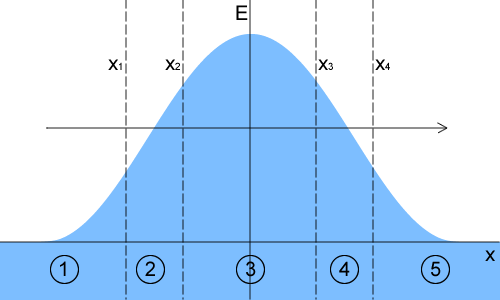
\includegraphics[scale=0.6]{images/wkb-barrier}}
			\caption{Diagram showing a smooth potential barrier in graphene with the the function $u\left(x\right)=1/\cosh(x)$. The four turning points $x_{1,2,3,4}$ and the five independent barrier regions have been labelled.}
			\label{fig:wkb-barrier}
		\end{figure}

		Unlike the Schr{\" o}dinger WKB barrier the graphene graphene barrier has four turning points. The four turning points are obtained from the requirement that $p_{x}=0$ at a turning point. The effect of having four turning points is that the graphene barrier acts as a double Schr{\" o}dinger barrier, which allows the comparison of the graphene wave-functions to standard Schr{\" o}dinger functions in order to derive a transfer matrix. Having a double barrier also allows bound states to be found in a similar way to the Schr{\" o}dinger barriers, which can lead to density of states and conductivity.

		As graphene allows transport via electrons and holes the regions 1,3 and 5 in Figure \ref{fig:wkb-barrier} are oscillatory wave-functions. In regions 2 and 4 exponential growth and decay occurs.
	
		The graphene Hamintonian as given in \cite{b1} can be written in matrix form as:
		\begin{align}
			\hat{H_{g}}=
			\left[\begin{array}{cc}
				u\left(x\right)&v_{f}\left(\hat{p}_{x}-i\hat{p}_{y}\right)\\
				v_{f}\left(\hat{p}_{x}+i\hat{p}_{y}\right)&u\left(x\right)
			\end{array}\right]
		\end{align}
		When applied to the Dirac equation, this can be converted to a dimensionless system:
		\begin{align}
			\left[\begin{array}{cc}
				U\left(x\right)&h\left(-i\frac{\partial}{\partial x}-\frac{\partial}{\partial y}\right)\\
				h\left(-i\frac{\partial}{\partial x}+\frac{\partial}{\partial y}\right)&U\left(x\right)
			\end{array}\right]
			\left[\begin{array}{cc}
				u\\
				v
			\end{array}\right]
			=0
		\end{align}
		Here the constant $h=\hbar v_{f}/U_{0}D$ has been introduced. The constant $U_{0}$ is defined as the maximum height of the barrier, $U(x)$ is the rescaled potential function so that $u\left(x\right)=U_{0}U\left(x\right)$ and $D$ is the size of the barrier in the $x$ dimension. This can then be reduced to the one dimensional system by requiring that the barrier only exists in the $x$ direction. With this condition the wave-function becomes separable and must be of the form:
		\begin{equation}
			\psi\left(x,y\right)=f\left(x\right)e^{\frac{i}{h}p_{y}y}
		\end{equation}
		Applying this wave-function to the Dirac system will remove the $y$ dependence, simplifying the system to:
		\begin{align}
			\left[\begin{array}{cc}
				U\left(x\right)&-ih\frac{\partial}{\partial x}-ip_{y}\\
				-ih\frac{\partial}{\partial x}+ip_{y}&U\left(x\right)
			\end{array}\right]
			\left[\begin{array}{cc}
				u\\
				v
			\end{array}\right]
			=0
		\end{align}
		This one dimensional reduced system will be used throughout this chapter.
%%%%%
%%%%%
%%%%%
		\section{WKB Solutions in a Classically Allowed Domain}
		\label{WKB Potential Barrier - WKB Solutions in a Classicaly Allowed Domain}
			Here the semiclassical wave-functions will be derived, these wave-functions take the form of an exponent of the action and are only valid away from the turning points. The valid regions are labelled as regions 1, 3 and 5 on Figure \ref{fig:wkb-barrier}. Solutions should be of the form:
			\begin{align}
				\psi=
				 e^{\frac{i}{h}s\left(x\right)}\sum\limits_{j=0}^\infty\left(\frac{h}{i}\right)^{j}
				\left[\begin{array}{cc}
					u\\
					v
				\end{array}\right]
				= e^{\frac{i}{h}s\left(x\right)}\sum\limits_{j=0}^\infty\left(\frac{h}{i}\right)^{j}\psi_{j}\left(x\right)
			\end{align}
			To find the values of $s\left(x\right)$ and $\psi_{0}$ the Dirac system in the zero-th order of $h$ can be used.
			\begin{equation}
				\left(\hat{H}-EI\right)\psi=0
			\end{equation}
			Where $\hat{H}$ is the reduced Hamiltonian and $I$ is the identity matrix.
			\begin{align}
				\hat{H}=
				\left[\begin{array}{cc}
					U\left(x\right)&-ih\frac{\partial}{\partial x}-ip_{y}\\
					-ih\frac{\partial}{\partial x}+ip_{y}&U\left(x\right)
				\end{array}\right]
				\hspace{1cm}
				I=
				\left[\begin{array}{cc}
					1&0\\
					0&1
				\end{array}\right]
			\end{align}
			Using these matricies the Dirac system can be expressed in matrix form:
			\begin{equation}
				\left[\begin{array}{cc}
					U\left(x\right)-E&-ih\frac{\partial}{\partial x}-ip_{y}\\
					-ih\frac{\partial}{\partial x}+ip_{y}&U\left(x\right)-E
				\end{array}\right]
				\left[\begin{array}{cc}
					u\\
					v
				\end{array}\right] e^{\frac{i}{h}s\left(x\right)}=0
			\end{equation}
			Expressing this as simultaneous equations, the unknown wave-function components can be expressed as:
			\begin{equation}
				u=-\frac{s'\left(x\right)-ip_{y}}{U\left(x\right)-E}v
			\end{equation}
			Substituting this back into the system of simultaneous equations results in an expression for $s\left(x\right)$:
			\begin{align}
				s'\left(x\right)^{2}&=\left(E-U\left(x\right)\right)^{2}-p_{y}^{2}\\
				s'\left(x\right)&=\pm\sqrt{\left(E-U\left(x\right)\right)^{2}-p_{y}^{2}}\\
				s'\left(x\right)&=p_{x}
			\end{align}
			The unknown wave-function components can then be obtained by finding the eigenvectors of the Hamiltonian.
			\begin{equation}
			He_{i}=\lambda_{i}e_{i},\hspace{1cm}i=1,2\hspace{1cm}\lambda_{i}=U\left(x\right)\pm p\hspace{1cm}i=1,2
			\end{equation}
			The eigenvectors are then:
			\begin{equation}
				e_{1}=\frac{1}{\sqrt{2}}\left[\begin{array}{cc}
					1\\
				e^{i\theta}
				\end{array}\right]
				\hspace{1cm}
				e_{2}=\frac{1}{\sqrt{2}}\left[\begin{array}{cc}
					1\\
					-e^{i\theta}
				\end{array}\right]
			\end{equation}
			where:
			\begin{equation}
				e^{i\theta}=\frac{p_{x}+ip_{y}}{p}\\
			\end{equation}
			For the zero-th order the full wave-function is of the form:
			\begin{gather}
				\psi_{0}=\sigma^{\left(0\right)}\left(x\right)e_{1}
			\end{gather}
			where $\sigma^{\left(0\right)}\left(x\right)$ is an unknown amplitude. Solvability of the Dirac system in the first order is needed to obtain this unknown amplitude. The Dirac system in the first order of $h$ can be obtained from:
			\begin{equation}
				\left(\hat{H}-EI\right)\left(-ih\psi_{1}+\psi_{0}\right) e^{\frac{i}{h}s\left(x\right)}=0
			\end{equation}
			Expressing this in matrix form:
			\begin{align}
				-ih
				\left[\begin{array}{cc}
					U\left(x\right)&-ih\frac{\partial}{\partial x}-ip_{y}\\
					-ih\frac{\partial}{\partial x}+ip_{y}&U\left(x\right)
				\end{array}\right]
				e^{\frac{i}{h}s\left(x\right)}\psi_{1}
				&=
				\left[\begin{array}{cc}
					U\left(x\right)&-ih\frac{\partial}{\partial x}-ip_{y}\\
					-ih\frac{\partial}{\partial x}+ip_{y}&U\left(x\right)
				\end{array}\right]
				e^{\frac{i}{h}s\left(x\right)}\psi_{0}
			\end{align}
			Removing terms not of the order $h^{1}$ produces:
			\begin{align}
				\left[\begin{array}{cc}
					U\left(x\right)-E&p_{x}-ip_{y}\\
					p_{x}+ip_{y}&U\left(x\right)-E
				\end{array}\right]
				\psi_{1}&=
				\left[\begin{array}{cc}
					0&-\frac{\partial}{\partial x}\\
					-\frac{\partial}{\partial x}&0
				\end{array}\right]
				\psi_{0}
			\end{align}
			The system can be expressed as:
			\begin{equation}
				H\psi_{1}=-R\psi_{0}
			\end{equation}
			In a more general from:
			\begin{equation}
				\left(H-EI\right)\psi_{j}=-R\psi_{j-1},\hspace{1cm}j>0
			\end{equation}
			Where the matrix $R$ is defined as:
			\begin{equation}
				R=
				\left[\begin{array}{cc}
					0&\frac{\partial}{\partial x}\\
					\frac{\partial}{\partial x}&0
				\end{array}\right],
			\end{equation}
			Solvability of the first order Dirac system requires the orthogonality condition \cite{b31}:
			\begin{gather}
				e^{*}_{1}\cdot R\left(\sigma e_{1}\right)=0
			\end{gather}
			Which results in the transport equation:
			\begin{gather}
				\frac{\partial\sigma}{\partial x}\left(e^{i\theta}+e^{-i\theta}\right)+\sigma\frac{\partial e^{i\theta}}{\partial x}=0
			\end{gather}
			With the solution:
			\begin{gather}
				\sigma=\frac{c}{\sqrt{2\cos(\theta)}}e^{-\frac{i\theta}{2}}
			\end{gather}
			Which results in the wave-function:
			\begin{align}
				\psi=&
				\left[\begin{array}{cc}
					u\\
					v
				\end{array}\right]
				= e^{\frac{i}{h}s\left(x\right)}\psi_{0}\left(x\right)=e^{\frac{i}{h}\int p_{x}dx}\sigma^{\left(0\right)}\left(x\right)e_{1}\\
				=&\frac{e^{\frac{i}{h}\int p_{x}dx}}{\sqrt{e^{2i\theta}+1}}\frac{c}{\sqrt{2}}
				\left[\begin{array}{cc}
					1\\
					e^{i\theta}
				\end{array}\right]
			\end{align}
%%%%%
%%%%%
%%%%%
		\section{WKB Solutions in a Classically Disallowed Domain}
		\label{WKB Potential Barrier - WKB Solutions in a Classicaly Disallowed Domain}
			These wave-functions are to be used between the sets of turning points, or in the Shr{\" o}dinger analogy, inside the potential barrier. The decaying solutions should be of the form:
			\begin{align}
				\psi=
				 e^{\frac{1}{h}s\left(x\right)}\sum\limits_{j=0}^\infty\left(\frac{h}{i}\right)^{j}
				\left[\begin{array}{cc}
					u\\
					v
				\end{array}\right]
				= e^{\frac{1}{h}s\left(x\right)}\sum\limits_{j=0}^\infty\left(\frac{h}{i}\right)^{j}\psi_{j}\left(x\right)
			\end{align}
			The same method for the classically allowed region can be applied to the classically disallowed region. Using the graphene Hamiltonian the classical action becomes:
			\begin{gather}
				H=
				\left[\begin{array}{cc}
					U\left(x\right)&iq-ip_{y}\\
					iq+ip_{y}&U\left(x\right)
				\end{array}\right]
				\hspace{1cm}
				s'\left(x\right)=q=\sqrt{\left(U\left(x\right)-E\right)^{2}-p_{y}^{2}}
			\end{gather}
			The eigenvalues in the classically disallowed region are obtained from the matrix Hamiltonian:
			\begin{equation}
				\lambda_{i}=U\left(x\right)\pm\sqrt{p_{y}^{2}-q^{2}}
				\hspace{1cm}
				i=1,2
			\end{equation}
			With the eigenvalues the eigenvectors can be obtained:
			\begin{align}
				e_{1}=\frac{1}{\sqrt{1+|\kappa|^{2}}}\left[\begin{array}{cc}
					1\\
					i\kappa_{\pm}
				\end{array}\right]\approx
				\left[\begin{array}{cc}
					\cos(\phi)\\
					i\sin(\phi)
				\end{array}\right]
				\hspace{1cm}
				e_{2}=\frac{1}{\sqrt{1+|\kappa|^{2}}}\left[\begin{array}{cc}
					1\\
					-i\kappa_{\pm}
				\end{array}\right]\approx
				\left[\begin{array}{cc}
					\cos(\phi)\\
					-i\sin(\phi)
				\end{array}\right]	
			\end{align}
			where:
			\begin{equation}
				-\frac{\pi}{4}<\phi<\frac{\pi}{4}\hspace{1cm}\kappa_{\pm}=\frac{\pm q+p_{y}}{E-U\left(x\right)}\approx \tan(\phi)
			\end{equation}
			For the zero-th order the full wave-function is of the form:
			\begin{gather}
				\psi_{0}=\sigma^{\left(0\right)}\left(x\right)e_{1}
			\end{gather}
			Where $\sigma^{\left(0\right)}\left(x\right)$ is an unknown amplitude. Solvability of the Dirac system in the first order:
			\begin{gather}
				\left(H-EI\right)\psi_{1}=-R\psi_{0}
			\end{gather}
			Requires the orthogonality condition:
			\begin{gather}
				l_{1}^{*}\cdot R\left(\sigma e_{1}\right)=0
			\end{gather}
			Here $l_{1}^{*}$ is the eigenvector of the Hamiltonian $H^{*}$, which are defined as:
			\begin{align}
				H^{*}=
				\left[\begin{array}{cc}
					U\left(x\right)&-iq+ip_{y}\\
					-iq-ip_{y}&U\left(x\right)
				\end{array}\right]
				\hspace{1cm}
				l_{1}^{*}=
				\left[\begin{array}{cc}
					\sin(\phi)\\
					-i\cos(\phi)
				\end{array}\right]	
			\end{align}
			Which results in the transport equation:
			\begin{gather}
				\frac{\partial\sigma^{\left(0\right)}}{\partial x}-\sigma^{\left(0\right)}\tan(2\phi)\frac{\partial\phi}{\partial x}=0
			\end{gather}
			With the solution:
			\begin{gather}
				\frac{c}{\sqrt{\cos(2\phi)}}
			\end{gather}
			Which can be expressed as:
			\begin{gather}
				\frac{c}{\sqrt{-\cos(2\phi)}}=c\sqrt{\frac{1+\kappa_{\pm}^{2}}{\kappa_{\pm}^{2}-1}}
			\end{gather}
			Which results in the total wave-function:
			\begin{gather}
				\psi=\frac{c}{\sqrt{\kappa_{\pm}^{2}-1}}e^{\frac{1}{h}\int qdx}
				\left[\begin{array}{cc}
					1\\
					i\kappa_{\pm}
				\end{array}\right]
			\end{gather}
%%%%%
%%%%%
%%%%%
	\section{Left Slope Tunnelling}
	\label{WKB Potential Barrier - Left-Slope Tunneling}
		As the graphene barrier is represented by two Schr{\" o}dinger barriers, a single barrier must first be modelled. The graphene wave-functions can then be compared to the Schr{\" o}dinger result in order to obtain a graphene result.	The graphene WKB solutions derived earlier must be combined with their respective reflected components. These wave-functions then take the form:
		\begin{align}
			\psi_{1}&=\frac{e^{\frac{i}{h}\int^{x}_{x_{1}} p_{x}dx}}{\sqrt{e^{2i\theta^{+}}+1}}\frac{a_{1}}{\sqrt{2}}
			\left[\begin{array}{cc}
				1\\
				e^{i\theta^{+}}
			\end{array}\right]+
			\frac{e^{-\frac{i}{h}\int^{x}_{x_{1}} p_{x}dx}}{\sqrt{e^{2i\theta^{-}}+1}}\frac{a_{2}}{\sqrt{2}}
			\left[\begin{array}{cc}
				1\\
				e^{i\theta^{-}}
			\end{array}\right]\\
			\psi_{2}&=\frac{e^{-\frac{1}{h}\int^{x}_{x_1} qdx}}{\sqrt{\kappa_{+}^{2}-1}}c_{1}
			\left[\begin{array}{cc}
				1\\
				i\kappa_{+}
			\end{array}\right]
			+\frac{e^{\frac{1}{h}\int^{x}_{x_1} qdx}}{\sqrt{\kappa_{-}^{2}-1}}c_{2}
			\left[\begin{array}{cc}
				1\\
				i\kappa_{-}
			\end{array}\right]\\
			\psi_{3}&=\frac{e^{\frac{i}{h}\int^{x}_{x_{2}} p_{x}dx}}{\sqrt{e^{2i\theta^{+}}+1}}\frac{d_{1}}{\sqrt{2}}
			\left[\begin{array}{cc}
				1\\
				e^{i\theta^{+}}
			\end{array}\right]+
			\frac{e^{-\frac{i}{h}\int^{x}_{x_{2}} p_{x}dx}}{\sqrt{e^{2i\theta^{-}}+1}}\frac{d_{2}}{\sqrt{2}}
			\left[\begin{array}{cc}
				1\\
				e^{i\theta^{-}}
			\end{array}\right]
			\label{wkb-wave-functions-slope}
		\end{align}
		where:
		\begin{equation}
			e^{i\theta^{\pm}}=\frac{\pm p_{x}+ip_{y}}{E-U\left(x\right)}
			\hspace{1cm}
			\kappa_{\pm}=\frac{\pm q+p_{y}}{E-U\left(x\right)}
		\end{equation}
		In order to match the graphene equations for each region, a change of variables and an effective Shr{\" o}dinger equation should be derived from the Dirac system. Using the definitions:
		\begin{equation}
			U\left(x\right)-E=\epsilon\hspace{1cm}\alpha\left(\epsilon\right)=\frac{\partial\epsilon}{\partial x}\hspace{1cm}\hat{p}_{x}=-ih\frac{\partial}{\partial x}
		\end{equation}
		The Hamiltonian can be represented in the Dirac equation as:
		\begin{align}
			\left[\begin{array}{cc}
				\epsilon&-ih\alpha\frac{\partial}{\partial\epsilon}-ip_{y}\\
				-ih\alpha\frac{\partial}{\partial\epsilon}+ip_{y}&\epsilon
			\end{array}\right]
			\left[\begin{array}{cc}
				u\\
				v
			\end{array}\right]=0
		\end{align}
		Using the substitution:
		\begin{equation}
			W=\frac{u+v}{2}
			\hspace{1cm}
			V=\frac{u-v}{2}
		\end{equation}
		creates the system of simultaneous equations:
		\begin{align}
			\epsilon V+ih\alpha\frac{\partial}{\partial\epsilon}V-ip_{y}W&=0\\
			\epsilon W-ih\alpha\frac{\partial}{\partial\epsilon}W+ip_{y}V&=0
		\end{align}
		Solving these equations will allow the quantity $V$ to be eliminated, which leads to the equation:
		\begin{equation}
			h^{2}W''+W\left(\frac{\epsilon^{2}-p_{y}^{2}}{\alpha^{2}}+\frac{ih}{\alpha}\right)+h^{2}\frac{\alpha'}{\alpha}W'=0
			\label{WKB-W}
		\end{equation}
		Here the prime notation denotes differentiation with respect to $\epsilon$. Using the second change of variable:
		\begin{gather}
			W=\frac{\omega}{\sqrt{\alpha}}
		\end{gather}
		Equation (\ref{WKB-W}) takes the form:
		\begin{equation}
			h^{2}\omega''+\omega\left(\frac{\epsilon^{2}-p_{y}^{2}}{\alpha^{2}}+\frac{ih}{\alpha}+h^{2}\frac{1}{4}\alpha^{-2}\alpha'^{2}-h^{2}\frac{1}{2}\alpha^{-1}\alpha''\right)=0
		\end{equation}
		with the identities:
		\begin{align}
			\left(\ln(\alpha)\right)'=\alpha^{-1}\alpha'
			\hspace{1cm}
			\left(\ln(\alpha)\right)''=-\alpha^{-2}\alpha'^{2}+\alpha^{-1}\alpha''
		\end{align}
		Equation (\ref{WKB-W}) becomes:
		\begin{equation}
			h^{2}\omega''+\omega\left(\frac{\epsilon^{2}-p_{y}^{2}}{\alpha^{2}}+\frac{ih}{\alpha}-\frac{1}{4}h^{2}\left(\ln(\alpha)\right)'^{2}-\frac{1}{2}h^{2}\left(\ln(\alpha)\right)''\right)=0
		\end{equation}
		Terms with $h^{2} \ln(\alpha)$ may be considered as too small and removed, resulting in:
		\begin{equation}
			h^{2}\omega''+\omega\left(\frac{\epsilon^{2}-p_{y}^{2}}{\alpha^{2}}+\frac{ih}{\alpha}\right)=0
			\label{WKB-w}
		\end{equation}
		The wave-functions in Equation (\ref{wkb-wave-functions-slope}) must also undergo the change of variables:
		\begin{equation}
			\omega=\sqrt{\alpha}\left(\frac{u+v}{2}\right)
		\end{equation}
		The change in variables produce the wave-functions:
		\begin{align}
			\omega_{1}&=\frac{1}{2}\sqrt{\frac{\alpha}{2}}\left(a_{1}e^{\frac{i}{h}\int^{x}_{x_{1}} \frac{\sqrt{\epsilon^{2}-p_{y}^{2}}}{\alpha}d\epsilon}\frac{A^{+}}{P^{+}}+a_{2}e^{-\frac{i}{h}\int^{x}_{x_{1}} \frac{\sqrt{\epsilon^{2}-p_{y}^{2}}}{\alpha}d\epsilon}\frac{A^{-}}{P^{-}}\right)\\
			\omega_{2}&=\frac{\sqrt{\alpha}}{2}\left(c_{1}e^{-\frac{1}{h}\int^{x}_{x_1}\frac{\sqrt{p_{y}^{2}-\epsilon^{2}}}{\alpha}d\epsilon}\frac{B^{+}}{Q^{+}}+c_{2}e^{\frac{1}{h}\int^{x}_{x_1}\frac{\sqrt{p_{y}^{2}-\epsilon^{2}}}{\alpha}d\epsilon}\frac{B^{-}}{Q^{-}}\right)\\
			\omega_{3}&=\frac{1}{2}\sqrt{\frac{\alpha}{2}}\left(d_{1}e^{\frac{i}{h}\int^{x}_{x_{2}} \frac{\sqrt{\epsilon^{2}-p_{y}^{2}}}{\alpha}d\epsilon}\frac{A^{+}}{P^{+}}+d_{2}e^{-\frac{i}{h}\int^{x}_{x_{2}} \frac{\sqrt{\epsilon^{2}-p_{y}^{2}}}{\alpha}d\epsilon}\frac{A^{-}}{P^{-}}\right)
			\label{WKB-change-variable}
		\end{align}
		Where the definitions have been introduced:
		\begin{align}
			A^{\pm}&=1-\frac{\pm p_{x}+ip_{y}}{\epsilon}
			\hspace{1cm}
			P^{\pm}=\sqrt{1+\left(\frac{\pm p_{x}+ip_{y}}{\epsilon}\right)^{2}}\\
			B^{\pm}&=1-i\frac{\pm q+p_{y}}{\epsilon}
			\hspace{1cm}
			Q^{\pm}=\sqrt{\left(\frac{\pm q+p_{y}}{\epsilon}\right)^{2}-1}
		\end{align}
		These wave-functions must then match the solutions to the Equation (\ref{WKB-w}). The solutions to Equation (\ref{WKB-w}) in regions 1 and 3 should be of the form:
		\begin{equation}
			\omega_{1,3}=\omega^{+}e^{\frac{i}{h}s}+\omega^{-}e^{-\frac{i}{h}s}
		\end{equation}
		By substituting $\omega=\omega^{+}e^{\frac{i}{h}s}$ into Equation (\ref{WKB-w}) and only considering the zero-th order of $h$ terms, the action can be obtained:
		\begin{equation}
			s'=\frac{\sqrt{\epsilon^{2}-p_{y}^{2}}}{\alpha}
		\end{equation}
		Then by considereing only $h$ order terms and using the definition of $s'$, $\omega^{+}$ becomes:
		\begin{equation}
			\omega^{+}=\frac{\sqrt{\alpha}}{\left(\epsilon^{2}-p_{y}^{2}\right)^{\frac{1}{4}}}\frac{1}{D^{-}}
			\hspace{1cm}
			D^{\pm}=\sqrt{\frac{\epsilon+\sqrt{\epsilon^{2}-p_{y}^{2}}}{\pm p_{y}}}
		\end{equation}
		Similarly the value of $\omega^{-}$ can be obtained with $\omega=\omega^{-}e^{-\frac{i}{h}s}$ and Equation (\ref{WKB-w}):
		\begin{equation}
			\omega^{-}=\frac{\sqrt{\alpha}}{\left(\epsilon^{2}-p_{y}^{2}\right)^{\frac{1}{4}}}D^{-}
		\end{equation}
		The solutions in region 2 are then required to be of the form:
		\begin{equation}
			\omega_{2}=\omega^{+}e^{\frac{1}{h}s}+\omega^{-}e^{-\frac{1}{h}s}
		\end{equation}
		Again using Equation (\ref{WKB-w}) the zero order terms of the small parameter $h$ will provide the action in region 2:
		\begin{equation}
			s'=\frac{\sqrt{p_{y}^{2}-\epsilon^{2}}}{\alpha}
		\end{equation}
		The $h$ order terms, with $\omega=\omega^{+}e^{\frac{1}{h}s}$ then produce:
		\begin{equation}
			\omega^{+}=\frac{\sqrt{\alpha}}{\left(p_{y}^{2}-\epsilon^{2}\right)^{\frac{1}{4}}}e^{-\frac{1}{2}i\arcsin\left(\frac{\epsilon}{p_{y}}\right)-\frac{i\pi}{4}}
		\end{equation}
		Then with the reflected term $\omega=\omega^{-}e^{-\frac{1}{h}s}$, the value for $\omega^{-}$ becomes:
		\begin{equation}
			\omega^{-}=\frac{\sqrt{\alpha}}{\left(p_{y}^{2}-\epsilon^{2}\right)^{\frac{1}{4}}}e^{\frac{1}{2}i\arcsin\left(\frac{\epsilon}{p_{y}}\right)+\frac{i\pi}{4}}
		\end{equation}
		Details of how these expressions were obtained can be found in the appendix Section \ref{Appendix-WKB-Solutions}. The comparisons to the wave-functions in Equation (\ref{WKB-change-variable}) from the change in variables can be found in the appendix Section \ref{Appendix-Matching-Variables}. The full solutions to Equation (\ref{WKB-w}) can now be written as:
		\begin{align}
			\omega_{1}&=\frac{1}{2\left(\epsilon^{2}-p_{y}^{2}\right)^{\frac{1}{4}}}\sqrt{\frac{p_{y}\alpha}{2}}\left(\sgn(p_{y})a_{1}\frac{1}{D^{-}}e^{\frac{i}{h}\int^{\epsilon}_{-p_{y}}\frac{\sqrt{\epsilon^{2}-p_{y}^{2}}}{\alpha}d\epsilon}-ia_{2}D^{-}e^{-\frac{i}{h}\int^{\epsilon}_{-p_{y}}\frac{\sqrt{\epsilon^{2}-p_{y}^{2}}}{\alpha}d\epsilon}\right)\\
			\omega_{2}&=\frac{\sgn(p_{y})\sqrt{p_{y}\alpha}}{2\left(p_{y}^{2}-\epsilon^{2}\right)^{\frac{1}{4}}}\left(ic_{1}e^{-\frac{1}{h}\int^{\epsilon}_{-p_{y}}\frac{\sqrt{p_{y}^{2}-\epsilon^{2}}}{\alpha}d\epsilon+\frac{1}{2}i\arcsin\left(\frac{\epsilon}{p_{y}}\right)+\frac{i\pi}{4}}+c_{2}e^{\frac{1}{h}\int^{\epsilon}_{-p_{y}}\frac{\sqrt{p_{y}^{2}-\epsilon^{2}}}{\alpha}d\epsilon-\frac{1}{2}i\arcsin\left(\frac{\epsilon}{p_{y}}\right)-\frac{i\pi}{4}}\right)\\
			\omega_{3}&=\frac{1}{2\left(\epsilon^{2}-p_{y}^{2}\right)^{\frac{1}{4}}}\sqrt{\frac{p_{y}\alpha}{2}}\left(-id_{1}\frac{1}{D^{+}}e^{\frac{i}{h}\int^{\epsilon}_{p_{y}}\frac{\sqrt{\epsilon^{2}-p_{y}^{2}}}{\alpha}d\epsilon}-\sgn(p_{y})d_{2}D^{+}e^{-\frac{i}{h}\int^{\epsilon}_{p_{y}}\frac{\sqrt{\epsilon^{2}-p_{y}^{2}}}{\alpha}d\epsilon}\right)
			\label{omega-final}
		\end{align}
		The solutions for the graphene WKB method should then be compared to the general WKB solutions in Section \ref{Appendix - Schrodinger WKB Barrier}. The relation between $\omega$ and $\bar{\omega}$ can be found:
		\begin{gather}
			e^{-\frac{i\pi}{4}}\omega=\sgn(p_{y})\frac{1}{2}\sqrt{p_{y}}\bar{\omega}
		\end{gather}
		Where the bar notation represents the WKB solutions from the Schr\"{o}dinger equation, details of this matching can be found in the appendix Section \ref{Appendix-Matching-Solutions}. In this way the constants $a$, $d$, $\bar{a}$ and $\bar{t}$ are related by:
		\begin{align}
			\bar{a}=\frac{1}{\sqrt{2}}
			\left[\begin{array}{cc}
				e^{-\frac{i\pi}{4}}		&	0\\
				0	&	-e^{\frac{i\pi}{4}}\sgn(p_{y})
			\end{array}\right]a\hspace{1cm}
			d=\sqrt{2}
			\left[\begin{array}{cc}
				-e^{-\frac{i\pi}{4}}\sgn(p_{y})	&	0\\
				0	&	-e^{\frac{i\pi}{4}}
			\end{array}\right]\bar{d}
		\end{align}
		Using these relations the transfer matrix derived for the Schr{\" o}dinger barrier can be converted to the graphene case. With $\bar{d}=\bar{T}\bar{a}$ the transfer matrix $T_{1}$ becomes:
		\begin{align}
			T_{1}=\left[\begin{array}{cc}
				\sgn(p_{y})\left(e^{\frac{1}{h}Q_{1}}-\frac{1}{4}e^{-\frac{1}{h}Q_{1}}\right)	&	-e^{\frac{1}{h}Q_{1}}-\frac{1}{4}e^{-\frac{1}{h}Q_{1}}\\
				-e^{\frac{1}{h}Q_{1}}-\frac{1}{4}e^{-\frac{1}{h}Q_{1}}	&	\sgn(p_{y})\left(e^{\frac{1}{h}Q_{1}}-\frac{1}{4}e^{-\frac{1}{h}Q_{1}}\right)
			\end{array}\right]
		\end{align}
		Where:
		\begin{align}
			Q_{1}=\frac{1}{h}\int^{p_{y}}_{-p_{y}}\frac{\sqrt{p_{y}^{2}-\epsilon^{2}}}{\alpha}d\epsilon=\frac{1}{h}\int^{x_{2}}_{x_{1}}\sqrt{p_{y}^{2}-\left(E-U\left(x\right)\right)^{2}}dx
		\end{align}
%%%%%
%%%%%
%%%%%
	\section{Total Transfer Matrix}
	\label{WKB Potential Barrier - Total Transfer Matrix}
		The total transfer matrix for a smooth barrier must include right slope tunnelling as well as the region between slopes. If the barrier is symmetrical the transfer matricies for the left and right slope are identical with a change in turning points. If the barrier is not symmetrical new turning points and $Q$ will have to be derived. The region between the barriers must also be considered. This was obtained in Section \ref{Appendix - Schrodinger WKB Barrier} for Schr\"{o}dinger barriers. Using the same method used for deriving the left slope transport, the region between barriers can be converted for use with the graphene case. Therefore this simply takes the form:
		\begin{equation}
			T_{3}=\left[\begin{array}{cc}
				e^{\frac{i}{h}P}&0\\
				0&e^{-\frac{i}{h}P}
			\end{array}\right]
		\end{equation}
		Where $P$ for the graphene case becomes:
		\begin{equation}
			P=\frac{1}{h}\int_{x_{2}}^{x_{3}}\sqrt{\left(U_{1}\left(x\right)-E\right)^2-p_{y}^{2}}dx
		\end{equation}
		To consider non-symmetrical barriers an expression for the right slope can easily be obtained from the left slope. Only the quantity $Q$ and the turning points need to be adjusted. The right slope is then represented by:
		\begin{equation}
			T_{2}=\left[\begin{array}{cc}
				\sgn(p_{y})\left(e^{\frac{1}{h}Q_{2}}-\frac{1}{4}e^{-\frac{1}{h}Q_{2}}\right)	&	-e^{\frac{1}{h}Q_{2}}-\frac{1}{4}e^{-\frac{1}{h}Q_{2}}\\
				-e^{\frac{1}{h}Q_{2}}-\frac{1}{4}e^{-\frac{1}{h}Q_{2}}	&	\sgn(p_{y})\left(e^{\frac{1}{h}Q_{2}}-\frac{1}{4}e^{-\frac{1}{h}Q_{2}}\right)
			\end{array}\right]
		\end{equation}
		with:
		\begin{equation}
			Q_{2}=\frac{1}{h}\int^{p_{y}}_{-p_{y}}\frac{\sqrt{p_{y}^{2}-\epsilon^{2}}}{\alpha}d\epsilon=\frac{1}{h}\int^{x_{4}}_{x_{3}}\sqrt{p_{y}^{2}-\left(E-U_{2}\left(x\right)\right)^{2}}dx
		\end{equation}
		From transfer matrix theory the transfer matrices for each region can be combined to find the total transfer matrix of the system. This means the total transfer matrix for a smooth graphene barrier is:
		\begin{equation}
			T_{T}=T_{2}T_{3}T_{1}
		\end{equation}
		Where the matrix elements are defined as:
		\begin{align}
			T_{11}&=2\cos(P)\left(e^{Q_{2}+Q_{1}}+\frac{1}{16}e^{-Q_{2}-Q_{1}}\right)-i\sin(P)\cosh(Q_{2}-Q_{1})\\
			T_{12}&=\sgn(p_{y})\left(2\cos(P)\left(-e^{Q_{2}+Q_{1}}+\frac{1}{16}e^{-Q_{2}-Q_{1}}\right)-i\sin(P)\sinh(Q_{2}-Q_{1})\right)\\
			T_{21}&=\sgn(p_{y})\left(2\cos(P)\left(-e^{Q_{2}+Q_{1}}+\frac{1}{16}e^{-Q_{2}-Q_{1}}\right)+i\sin(P)\sinh(Q_{2}-Q_{1})\right)\\
			T_{22}&=2\cos(P)\left(e^{Q_{2}+Q_{1}}+\frac{1}{16}e^{-Q_{2}-Q_{1}}\right)+i\sin(P)\cosh(Q_{2}-Q_{1})
		\end{align}
		The transmission probability through the system is then given by:
		\begin{equation}
			T=|t|^{2}=\frac{1}{|T_{22}|^{2}}
		\end{equation}
		Evaluating this with the graphene WKB transfer matrix produces:
		\begin{equation}
			T=\frac{1}{4\cos^{2}(P)\left(e^{Q_{2}+Q_{1}}+\frac{1}{16}e^{-Q_{2}-Q_{1}}\right)^{2}+\sin^{2}(P)\cosh^{2}(Q_{2}-Q_{1})}
			\label{wkb-T}
		\end{equation}
%%%%%
%%%%%
%%%%%
	\section{Bound states}
	\label{WKB Potential Barrier - Bound states}
		In the Schr{\" o}dinger case localised bound states can be found within a double barrier structure. It has been shown that a single graphene barrier is also capable of producing bound states \cite{b3}. In this model the bound states will be of oscillatory type between the two slopes and must decay exponentially as $x$ tends to infinity. Therefore by setting $T_{22}=0$, the bound states can be found for the system. For simplicity the case where $Q_{1}=Q_{2}$ will be examined, representing a symmetrical graphene barrier. 
		\begin{equation}
			2\cos(P)\left(e^{Q_{2}+Q_{1}}+\frac{e^{-Q_{2}-Q_{1}}}{16}\right)+i\sin(P)\cosh(Q_{2}-Q_{1})=0
		\end{equation}
		 With $Q_{1}=Q_{2}$ the matrix element $T_{22}$ is reduced to:
		\begin{equation}
			\cot(P)\left(e^{2Q_{1}}+\frac{e^{-2Q_{1}}}{16}\right)=0
		\end{equation}
		This condition is satisfied when:
		\begin{align}
			P=\pi\left(n+\frac{1}{2}\right)
		\end{align}
		This condition is similar to the Bohr-Sommerfeld condition seen in the Schr{\" o}dinger case. For a symmetrical barrier and the previous definition of $P$ this condition becomes:
		\begin{equation}
			\frac{1}{h}\int_{x_{2}}^{x_{3}}\sqrt{\left(U_{1}\left(x\right)-E\right)^2-p_{y}^{2}}dx=\pi\left(n+\frac{1}{2}\right)
			\label{wkb-bound-eq}
		\end{equation}
%%%%%
%%%%%
%%%%%
	\section{Results}
	\label{WKB Potential Barrier - Results}
		The results from the transmission can then be plotted with respect to dimensionless energy. The potential $U\left(x\right)=1/cosh\left(x\right)$ satisfies the condition of $U\left(x\right) \rightarrow 0$ when $x=\pm\infty$ making it suitable for testing this method. For simplicity, the barrier is symmetrical so that $Q_{1}=Q_{2}$. Values for each energy were then used with $U\left(x\right)=1/\cosh(x)$ to produce the four turning points:
		\begin{align}
			x=\pm \arccosh\left(\frac{1}{E \pm p_{y}}\right)
		\end{align}

		This then produces the transmission probability plot shown in Figure \ref{wkb-transmission}. With $p_{y}=0.25$ this plot shows peaks of perfect transmission and regions of $\sim$zero transmission probability, as expected for a graphene potential barrier with a $y$ component of momentum.
		\begin{figure}[h]
			\centerline{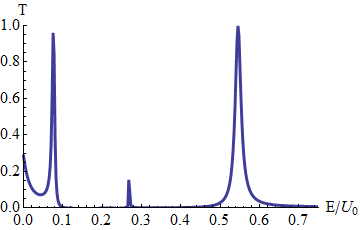
\includegraphics[scale=0.6]{images/wkb-transmission}}
			\caption{The transmission probability from Equation (\ref{wkb-T}) for potential barrier of type $U\left(x\right)=1/\cosh(x)$. Here the dimensionless variables $h=0.25$ and $p_{y}=0.25$.}
			\label{wkb-transmission}
		\end{figure}

		This definition of $U(x)$ is very well suited to model the smooth barrier, it meets all requirement for the model, as well as being symmetrical for simplicity. However, as the system is not identical to the rectangular barrier some variation is expected. Changing the function of $U\left(x\right)$ to something closer to a rectangular barrier would produce result more directly comparable. For this reason the function $U\left(x\right)=1/\cosh\left(x^{10}\right)$ was then tested. The result obtained with this potential is shown in Figure \ref{graphene-wkb-results-coshx10}.
		\begin{figure}[h]
			 \begin{subfigure}[h!]{0.5\textwidth}
				\centerline{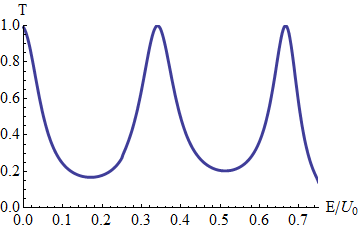
\includegraphics[scale=0.6]{images/graphene-wkb-results-coshx10}}
				\caption{}
			\end{subfigure}
			\begin{subfigure}[h!]{0.5\textwidth}
				\centerline{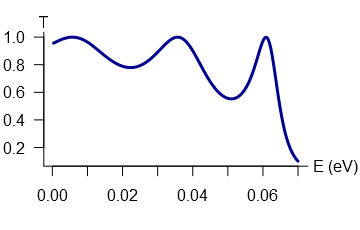
\includegraphics[scale=0.9]{images/wkb-comparison}}
				\caption{}
			\end{subfigure}
			\caption{(a) The transmission probability from Equation (\ref{wkb-T}) for potential barrier of type $U\left(x\right)=1/\cosh(x^{10})$. Here the dimensionless variables $h=0.25$ and $p_{y}=0.25$. (b) The transmission probability through a rectangular graphene potential barrier from Equation (\ref{eq:transmission}) with $d=100$ nm, $\theta_{a}=\pi /8$ and $V_{b}=0.1$ eV.}
			\label{graphene-wkb-results-coshx10}
		\end{figure}

		This function creates a potential which closely resembles the rectangular barrier. There is a large plateau at maximum barrier height, with shaper edges which reduce to zero at large values for $x$. This function widens the regions of high transmission probability and increases the minimum transmission probability to resemble the rectangular barrier at lower incident angles show in Figure \ref{graphene-wkb-results-coshx10} (b). This plot also shows the WKB system breaking down when energy approaches barrier height. This breakdown near barrier height is expected for this type of barrier, characterised in the rectangular case by the $\sgn(E-U)$ component of the wave-function.

		From the previously derived Bohr-Sommerfeld condition for graphene barriers, the bound states within a barrier with the potential $U(x)=1/\cosh(x)$  were also found and plotted in Figure \ref{wkb-energy-levels}. 
		\begin{figure}[h]
			\centerline{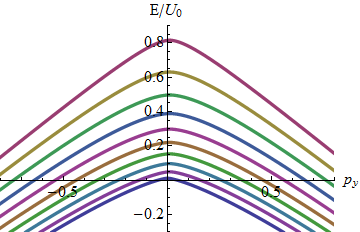
\includegraphics[scale=0.6]{images/wkb-energy-levels}}
			\caption{Bound states inside a potential barrier of type $U(x)=1/\cosh(x)$ calculated from the Bohr-Sommerfeld condition in Equation (\ref{wkb-bound-eq}). Here the dimensionless variables $h=0.25$ and $p_{y}=0.25$.}
			\label{wkb-energy-levels}
		\end{figure}

		This result perfectly recreates the result for the rectangular barrier in \cite{b3}, showing bound states occuring within the smooth barrier and showing a linear dependence on energy at large values of $p_{y}$.

		It is known that the occurence of bound states is dependent on the width of the barrier \cite{b3}. When the width of the rectangular barrier is increased, the number of bound states should increase. In order to verify that the WKB method will allow for this increase in bound states a function which will allow for a varied width must be used. The function:
		\begin{equation}
			U\left(x\right)=\frac{1}{2}\left(\tanh(x+a)-\tanh(x-a)\right)
		\end{equation}
		satisfies the previously defined criteria for suitable potentials. This function creates a plateau at barrier height which can be controlled with the parameter $a$. In this way the width of the barrier can easily be changed to test for an increase in number of bound states. The results for transmission probability with two values for $a$ are shown in Figure \ref{graphene-wkb-results-a1}.
		\begin{figure}[h]
			 \begin{subfigure}[h!]{0.5\textwidth}
				\centerline{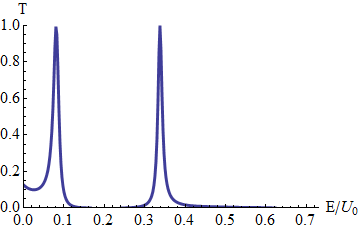
\includegraphics[scale=0.6]{images/graphene-wkb-results-a1}}
				\caption{a=1}
			\end{subfigure}
			\begin{subfigure}[h!]{0.5\textwidth}
				\centerline{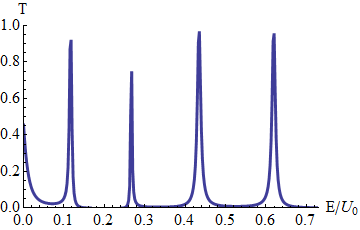
\includegraphics[scale=0.6]{images/graphene-wkb-results-a2}}
				\caption{a=2}
			\end{subfigure}
			\caption{The transmission probability through a graphene potential barrier with the potential $U\left(x\right)=\frac{1}{2}\left(\tanh(x+a)-\tanh(x-a)\right)$ calculated from Equation (\ref{wkb-T}) with a varying width $a$. Here the dimensionless variables $h=0.25$ and $p_{y}=0.25$.}
			\label{graphene-wkb-results-a1}
		\end{figure}

			The increase in number of peaks in Figure \ref{graphene-wkb-results-a1} clearly shows that the width of the barrier $a$ is controlling the resonances in a similar manner to the rectangular barrier. 
		\begin{figure}[h]
			\centerline{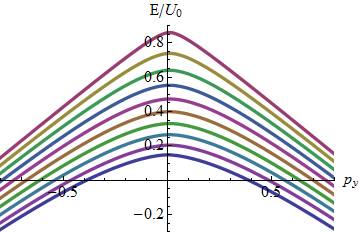
\includegraphics[scale=0.6]{images/graphene-wkb-energy-levels-a2}}
			\caption{Bound states inside a potential barrier of type $U\left(x\right)=\frac{1}{2}\left(\tanh(x+a)-\tanh(x-a)\right)$ calculated from the Bohr-Sommerfeld condition in Equation (\ref{wkb-bound-eq}). Here the dimensionless variables $h=0.25$ and $p_{y}=0.25$.}
			\label{graphene-wkb-energy-levels-a2}
		\end{figure}

		For bound states, the results in Figure \ref{graphene-wkb-energy-levels-a2} can be compared to that in Figure \ref{wkb-energy-levels}. This comparison clearly shows an increased number of bound states as barrier width increases as expected from the graphene rectangular barrier.
%\end{document}